\documentclass{article}

% if you need to pass options to natbib, use, e.g.:
\PassOptionsToPackage{numbers, compress}{natbib}
% before loading neurips_2020

% ready for submission
\usepackage{neurips_2020}

% to compile a preprint version, e.g., for submission to arXiv, add add the
% [preprint] option:
%     \usepackage[preprint]{neurips_2020}

% to compile a camera-ready version, add the [final] option, e.g.:
%     \usepackage[final]{neurips_2020}

% to avoid loading the natbib package, add option nonatbib:
     % \usepackage[nonatbib]{neurips_2020}

\usepackage[utf8]{inputenc} % allow utf-8 input
\usepackage[T1]{fontenc}    % use 8-bit T1 fonts
\usepackage{hyperref}       % hyperlinks
\usepackage{url}            % simple URL typesetting
\usepackage{booktabs}       % professional-quality tables
\usepackage{amsfonts}       % blackboard math symbols
\usepackage{nicefrac}       % compact symbols for 1/2, etc.
\usepackage{microtype}      % microtypography

% Personal imports
\nolinenumbers
\usepackage{natbib}
\bibliographystyle{unsrtnat}
\usepackage{graphicx}
\graphicspath{{./Figures/}}
% \usepackage{caption}
% \usepackage{multirow}
% \usepackage[normalem]{ulem}
% \useunder{\uline}{\ul}{}
\usepackage{placeins}

\title{Investigating Continual Learning Strategies in Nueral Networks}

% The \author macro works with any number of authors. There are two commands
% used to separate the names and addresses of multiple authors: \And and \AND.
%
% Using \And between authors leaves it to LaTeX to determine where to break the
% lines. Using \AND forces a line break at that point. So, if LaTeX puts 3 of 4
% authors names on the first line, and the last on the second line, try using
% \AND instead of \And before the third author name.

\author{
  Christopher Tam \\
  Department of Software Engineering\\
  Western University\\
  \texttt{ctam86@uwo.ca} \\
}

\begin{document}

\maketitle

\begin{abstract}
    This paper explores the role of continual learning strategies when neural networks are confronted with learning tasks sequentially. Our investigation measures forgetting with three factors in mind: the type of network architecture used, the continual learning scenario defined and the continual learning strategy implemented. This work is motivated by the theory that complementary learning systems are an essential ingredient in order to achieve lifelong learning, a theory put forward by McClelland et al. in 1998 \cite{mcclelland1995there}. Our results show that complementary learning systems provide significant improvements for memory retrieval and consolidation in neural networks, and provide the groundwork for further investigation in to the stability-plasticity dilemma. 
\end{abstract}

\section{Introduction}
As humans, we have the distinct ability to continually acquire knowledge throughout our lifetime. This ability, aptly referred to as lifelong learning, is enabled by a rich set of neurocognitive mechanisms that allow us to consolidate new information without forgetting previously learnt concepts. This is to say that the process of learning new information does not significantly interfere with our ability to recall old information. In contrast, current machine learning algorithms are unable to process novel streams of data without forgetting previously learnt patterns. This is referred to as \textit{catastrophic forgetting}. The problem of artificial intelligence (AI) systems learning over time by accommodating new knowledge and retaining previously learned patterns is referred to as \textit{continual learning}, and has been a long-standing challenge for machine learning and neural networks \cite{hassabis2017neuroscience}. In this project, we investigate continual learning strategies to overcome catastrophic forgetting in neural networks with three factors in mind: the type of network architecture used, the continual learning scenario defined and the continual learning strategy implemented. Specifically, we will be comparing multilayer perceptron to convolutional neural network architectures in the task-IL, domain-IL and class-IL continual learning scenarios using regularization, replay and hybrid continual learning strategies. 

\section{Background Work} \label{background}

\subsection{Catastrophic Forgetting and Continual Learning} \label{catastrophic_forgetting_and_CL}
A well known constraint for artificial and biological neural systems is the stability-plasticity dilemma \cite{mermillod2013stability}. This dilemma expresses the tradeoff between the integration of new knowledge and the stability required in order to prevent forgetting previously acquired knowledge in a neural system. On one hand, excessive plasticity will result in previously encoded information being constantly overwritten as learning takes place, whereas excessive stability will prevent the uptake of learning new data in the system. Between the two ends of the spectrum, McCloskey and Cohen \cite{mccloskey1989psychology} have found that artificial neural networks (henceforth referred to as neural networks) lean heavily towards plasticity, producing a phenomenon known as catastrophic forgetting \cite{mccloskey1989psychology}. Catastrophic forgetting is defined as the complete or significant forgetting of previously learned information by a neural network when exposed to new information, and has been demonstrated to be a general problem affecting many types of neural networks. For example, Richardson and Thomas \cite{richardson2008critical} showed catastrophic forgetting to be present in a variety of neural networks, from standard back-propagation networks to unsupervised self-organizing map networks to connectionist models of sentence acquisition. In artificial neural networks, catastrophic forgetting occurs when learning is prompted using a different distribution of data than what the network had previously been trained on. In this case, new data instances differ significantly from examples the network had previously observed. The new information causes the network to overwrite the shared representational resources holding the previously learned knowledge, producing a ‘catastrophic forgetting’ effect of those previously learned patterns. This problem has stood in the way of building lifelong learning systems, capable of learning from a continuous stream of information with information becoming progressively available over time and where the number of tasks to be learned are not predefined \cite{parisi2019continual}. In these systems, it is critical that the accommodation of new information should not be inhibited by the problem of catastrophic forgetting. 

\subsection{Three Continual Learning Scenarios} \label{three_CL_scenarios}
Research efforts towards continual learning has garnered plenty of attention and has resulted in a wide variety of experimental protocols being used. This has led to confusion, as some methods are shown to perform well in some certain experimental settings but dramatically fail in others. For example, the elastic weight consolidation algorithm presented by Kirkpatrick et al. \cite{kirkpatrick2017overcoming} claims state-of-the-art performance in it’s paper, but showed significant performance issues in the brain-inspired replay approach of ven de Ven et al. \cite{van2020brain}. In order to better compare methods for reducing catastrophic forgetting, this report will follow the three distinct scenarios for continual learning proposed by van de Ven and Tolias \cite{van2019three} (Figure \ref{fig:three_CL_scenarios}). This categorization focuses on the problem in which a single neural network is required to sequentially learn a series of tasks. Each scenario is distinguished by the task required and data available at test time, and will be presented in order of increasing difficulty in the following subsections.

\begin{figure}[h]
	\centering
    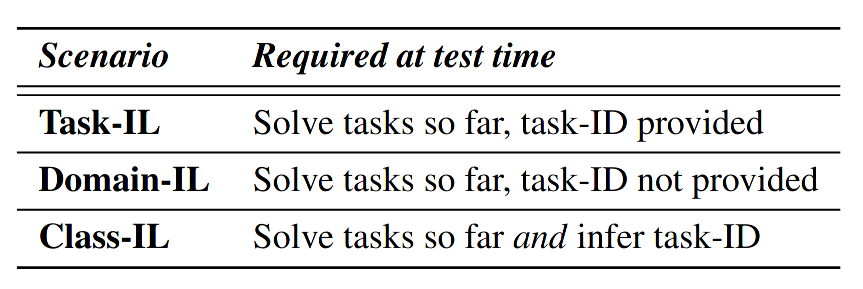
\includegraphics[width=0.60\linewidth]{three_CL_scenarios}
    \caption{Overview of the three continual learing scenarios proposed by \cite{van2019three}.}
	\label{fig:three_CL_scenarios}
\end{figure}

\subsubsection{Task-Incremental Learning (Task-IL)}
In the task-incremental learning scenario, the network is always informed about which task needs to be performed at test time. Given the availability of task identifiers at test time, it is possible to train a network with task-specific components. This enables architectures using a “multi-headed” output layer to be used, allowing the network to share its hidden resources but using task specific output units. 

\subsubsection{Domain-Incremental Learning (Domain-IL)}
In the domain-incremental learning scenario, the network is not informed about which task needs to be performed at test time. However, the network only needs to solve the task at hand and does not need to be able to infer which task group the task belongs to. This scenario is representative of problems where the structure of the tasks is always the same, but the input distribution is changing.

\subsubsection{Class-Incremental Learning (Class-IL)}
In the class-incremental learning scenario, the network must be able to solve a task as well as infer which class the task belongs to at test time. This scenario represents the most difficult problem in the categorization, and reflects the most common real-world problem of incrementally acquiring new knowledge. 

\subsection{Strategies for Continual Learning} \label{CL_stratgies}
In 1995, McClelland et al. proposed the Complementary Learning Systems theory \cite{mcclelland1995there}, which provided a basis for a computational framework modelling memory consolidation and retrieval. At the heart of this framework lies the interplay of episodic memory and semantic memory, which provided important insights into the mechanisms of memory consolidation in the absence of sensory input. Since then, many learning systems have taken inspiration from this framework in order to address the problem of catastrophic forgetting. As a result, there are several general categories which can be used to classify continual learning strategies. We may look to the Venn diagram of some of the most popular continual learning scenarios presented by Lesort et al. \cite{lesort2020continual}, for example. For the purpose of this paper, we will limit the discussion of strategies to those categories which are relevant to this project.

\begin{figure}[h]
	\centering
    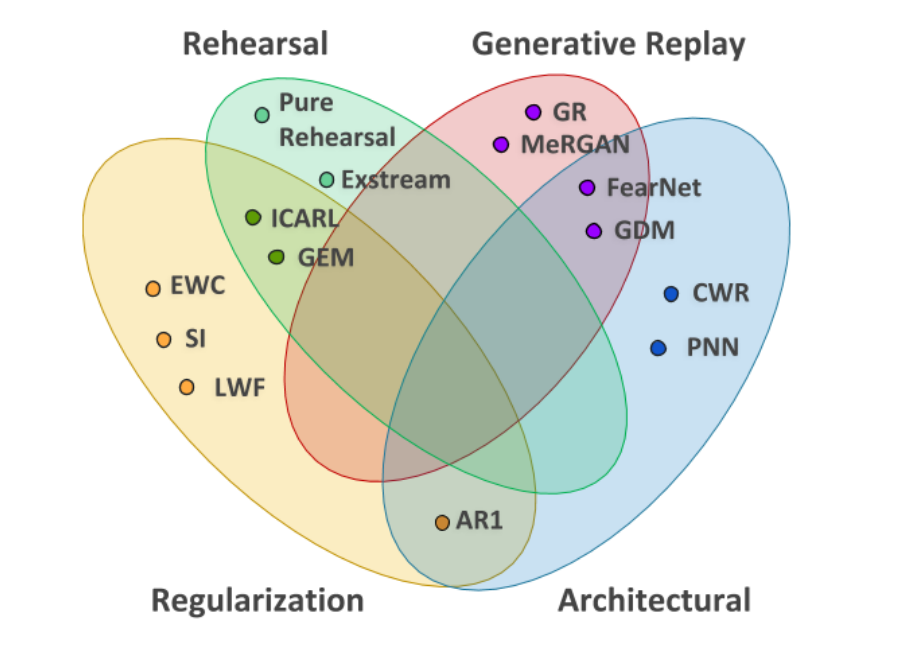
\includegraphics[width=0.60\linewidth]{CL_strategies_venn_diagram}
    \caption{Venn diagram of four of the most popular continual learning scenarios \cite{lesort2020continual}.}
	\label{fig:CL_strategies_venn_diagram}
\end{figure}

\subsubsection{Regularization Approaches}
Several approaches introduce a regularization term into the loss function in order to mitigate the effect of catastrophic forgetting. One way of doing this has been to regularize the network’s parameters during training on each new task, so as to constrain the movement of weights in a way that minimizes the amount of “forgetting”. This strategy has been implemented in the Elastic Weight Consolidation (EWC) \cite{kirkpatrick2017overcoming} and Synaptic Intelligence \cite{zenke2017continual} algorithms.  In both of these methods, estimates for the importance of parameters relevant to previously learned tasks are calculated and parameters are penalized proportional to their relative importance. This has the effect of slowing down learning for parts of the network which are important for previous tasks. Another class of regularization techniques is aimed at preventing activation drift primarily through means of knowledge distillation. One instance of this strategy is the Learning without Forgetting \cite{li2017learning} algorithm, which generates pseudo-data to train on using the input data of the current task and labelling it using the model trained on the previous tasks. The goal here is to prevent the representations of previous data from drifting too far away while learning new tasks.

\subsubsection{Replay Approaches} \label{replay_approaches}
Another approach for alleviating catastrophic forgetting is to store data from previous tasks. Replay methods keep a small number of “exemplars” or generate synthetic representations of the data previously encountered in order to prevent the forgetting of previous tasks. This approach has largely drawn on inspiration from the generative role of the hippocampus for the replay of previously encoded experiences. In 2017, Shin et al. \cite{shin2017continual} proposed a dual-model architecture consisting of a deep generative model and a task solver. Modelling the replay process of the hippocampus, their architecture sampled training data from previously learned experiences to generate pseudo-data to be interleaved with the data from new tasks. In this way, there was no requirement to explicitly revisit old training samples for experience replay and therefore reduced the cost requirements of working memory. More recently, Lorez-Paz and Ranzato \cite{lopez2017gradient} proposed Gradient Episodic Memory (GEM), a replay method which yields positive transfer of knowledge to previous tasks. GEM features an episodic memory storing a subset of previously seen examples from a given task. GEM requires far more memory than typical regularization approaches but has produced better results in single pass settings.

\section{Methodology} \label{methodology}

\subsection{Task Protocol}
Since the objective of this paper is to explore the differences between the three continual learning scenarios and to comprehensively compare the performances of the continual learning strategies discussed above, we selected a widely used task protocol for a basis of comparison. The permuted MNIST is a variation of the MNIST dataset, consisting of 70,000 handwritten digits from 0 to 9. 60,000 images are used for training, and 10,000 images are reserved for testing. Permuted MNIST differs from MNIST in that new tasks may be generated by permuting the pixels of each digit randomly. To generate the permuted images, the original 28x28 grey-scale images were randomly permuted so that the 784 pixels were randomly rearranged. The pixel values were transformed into a tensor and then normalized to a mean of 0.1307 and standard deviation of 0.3081. As a result, each new task can be considered a ten-way classification problem.

\subsection{Model Architectures}
To ensure a fair comparison, the same networks were used for all methods. Hyperparameters were tuned using a grid-search for each of the networks and the models yielding the highest average accuracy across all tasks were reported in the final comparison.

\subsubsection{Multilayer Perceptron Network}
A multilayer perceptron network with one hidden layer of 512 nodes was used. A ReLU nonlinearity was used as well as a dropout layer with a probability of 0.5. The network was optimized using stochastic gradient descent and minimized the multi-class cross entropy loss function. A summary of the multilayer perceptron network used is given in Figure \ref{fig:MLP}.

\begin{figure}[h]
	\centering
    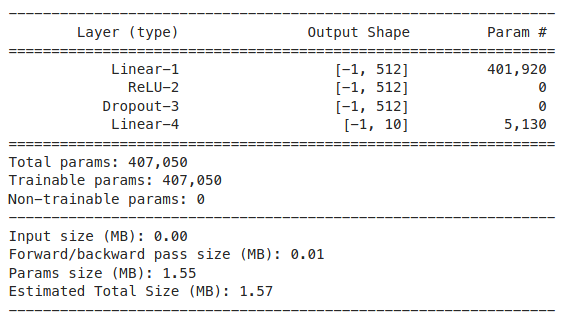
\includegraphics[width=0.60\linewidth]{MLP}
    \caption{Model summary of multilayer perceptron network.}
	\label{fig:MLP}
\end{figure}

\subsubsection{Convolutional Neural Network}
A convolutional neural network with two convolutional layers and two fully connected layers was used. For each convolutional layer, a kernel of size 5 and a ReLU nonlinearity was used. The two convolutional layers produced 6 and 16 output channels, respectively. Each convolutional layer was followed by a max pooling layer. In the two fully connected layers, 120 and 105 hidden units were used. The network was optimized using stochastic gradient descent and minimized the multi-class cross entropy loss function. A summary of the convolutional neural network is given in Figure \ref{fig:CNN}. 

\begin{figure}[h]
	\centering
    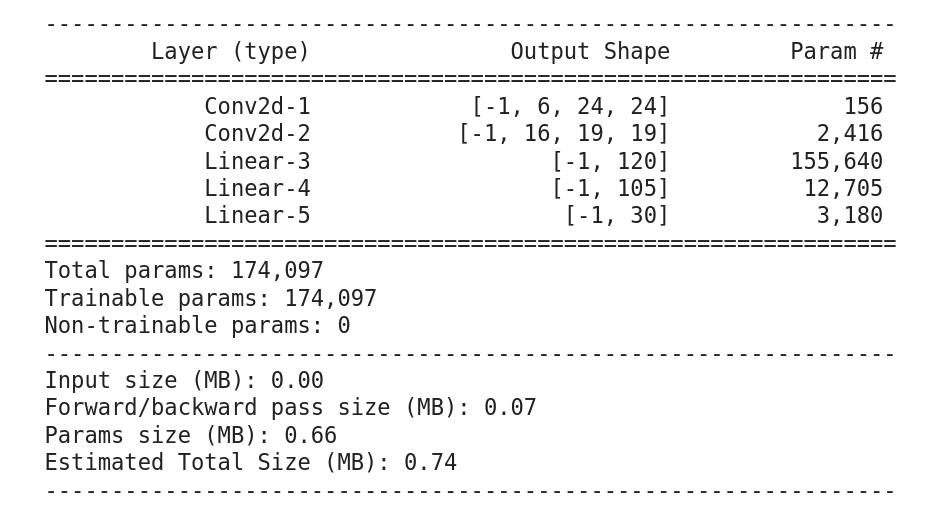
\includegraphics[width=0.60\linewidth]{CNN}
    \caption{Model summary of convolutional neural network.}
	\label{fig:CNN}
\end{figure}

\subsection{Continual Learning Scenarios}
As discussed in Section \ref{three_CL_scenarios}, we are interested in three continual learning scenarios. In order to provide a rigorous comparison, we will evaluate each scenario in a 3- and 10-task scenario. This should give us a better view of how each strategy generalizes to more tasks and will hopefully shine more light on stronger candidates. In this section we clearly define what each of these scenarios look like in the context of permuted MNIST. An overview of the scenarios under permuted MNIST is provided in Figure \ref{fig:CL_scenarios}.

\begin{figure}[h]
	\centering
    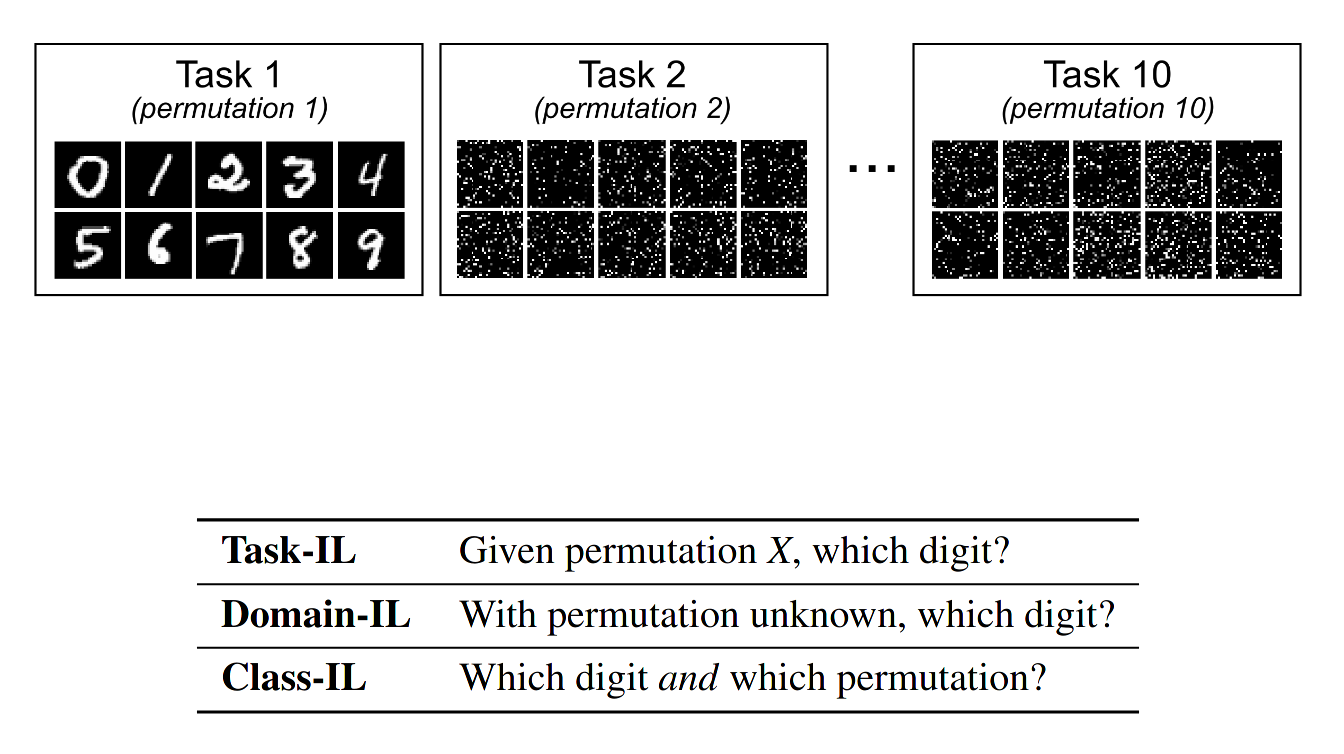
\includegraphics[width=0.60\linewidth]{CL_scenarios}
    \caption{Permuted MNIST according to Continual Learning scenarios \cite{van2019three}.}
	\label{fig:CL_scenarios}
\end{figure}

\subsubsection{Task-Incremental Learning (Task-IL)}
Under Task-IL, task identities are always known and shown at test time. Given an image and a task identity, the network must be able to correctly identify which digit the image represents. Setting up Task-IL involved assigning a progressive task identity to each of the permutations starting from “0”. A network was then consecutively trained on all tasks starting from task 0. At each step of the training loop (after training on each task) an evaluation loop would run to test the network’s ability to recall all previously seen tasks. Since the output of the network was always an integer between 0 and 9 inclusive, 10 units were used as output layer for architectures in the Task-IL scenario.

\subsubsection{Aside: Tasks vs. Experiences}
Before discussing the methodology behind implementing the Domain-IL and Class-IL scenarios, it will be helpful to distinguish between a task and an experience. These notions will make the intuition behind the implementation of these two scenarios much more clear. As shown in Figure \ref{fig:CL_scenarios}, task identities are not available at test time in Domain-IL and Class-IL. This is to say that task identities exist in both scenarios, but are merely not presented at test time. Tasks and experiences enable us to train a network on different task identities without exposing those identities at test time. Their primary difference is that networks are trained on experiences and are evaluated on tasks. Consider the following table for Class-IL with three permutations (identified as 0, 1 and 2): 

\begin{table}[h]
\centering
\caption{Tasks vs. Experiences}
\begin{tabular}{|c|c|}
\hline
\multicolumn{2}{|c|}{Class-IL} \\ \hline
Task        & Experience       \\ \hline
0           & 0                \\ \hline
0           & 1                \\ \hline
0           & 2                \\ \hline
\end{tabular}
\label{Tab:tasks_vs_experiences}
\end{table}

\subsubsection{Domain-Incremental Learning (Domain-IL)}
In Domain-IL, task identities are irrelevant at test time. Task identities are neither given nor expected to be inferred by the network. Given only an image, the network must be able to correctly identify which digit the image represents. We’ve already discussed how tasks and experiences allow us to train a network with different permutations without exposing their identities at test time. Under the permuted MNIST task protocol, a network will alway predict an integer between 0 and 9 (inclusive) for this scenario. The challenge is that for each evaluation step, a random bag of digits from all previously seen permutations will be presented. As such 10 units were used as the output layer for architectures under this scenario.

\subsubsection{Class-Incremental Learning (Class-IL)}
In Class-IL, task identities exist but are not provided at test time. Given an image, the network must be able to correctly identify which digit the image represents as well as correctly infer which permutation the image belongs to. This additional requirement prompted an adjustment to the labelling process of input and output classes. For each permutation, class labels were generated starting from the integer where the previous permutation ended. For instance, permutation 1 classes were labelled [0...9], permutations 2 classes were labelled [10...19], etc. At test time, these labels can be viewed as representing the m-th digit (ones column) from the n-th permutation (tens column). As a result, 3- and 10-times the number of units were used in the output layer for 3- and 10-task scenarios compared to the previous two scenarios. 

\subsection{Strategies}

\subsubsection{Naive}
In the naive strategy, a network is sequentially trained on all tasks. With each new task it encounters, the network fine-tunes it’s weights to fit the new data. This is where the most amount of catastrophic forgetting occurs, and will be used as a lower bound in our comparison.

\subsubsection{EWC}
The regularization approach selected for this project was Elastic Weight Consolidation (EWC) \cite{kirkpatrick2017overcoming}. In this strategy, a regularization term is added to the loss function which penalizes changes to parameters estimated to be important to previously learned tasks.  The regularization strength of the loss function is controlled by a hyperparameter $\lambda$, where
\[L_{total} = L_{current} + \lambda L_{regularization}\] 
We used grid search to find the optimal value of $\lambda$. 

\subsubsection{AGEM}
For the replay approach, we used the Average Gradient Episodic Memory (AGEM) \cite{chaudhry2018efficient} algorithm. AGEM is similar to the GEM algorithm discussed in \ref{replay_approaches}, but demands fewer memory requirements by storing the average gradient vector computed from the individual gradients of task loss for all previously seen tasks at each weight update. This is in contrast to GEM, where each task specific gradient vector has to be stored. The AGEM algorithm was tuned using two hyperparameters which varied the number of patterns to store in memory per experience, and number of patterns from each memory sample to consider when computing the reference gradient. The optimal values of these hyperparameters were found using grid search as well.

All strategies were trained for 3 iterations per task using the multi-class classification cross entropy classification loss. Networks were trained for 3 iterations per task using the SGD-optimizer with a learning rate of 0.01 and momentum of 0.9. The hyperparameter search for each of the methods is given in Table \ref{Tab:Hyperparameters}. We compared the continual learning strategies discussed above using the average test accuracy over all previously seen tasks.

\begin{table}[h]
\centering
\caption{Hyperparameter Values}
\begin{tabular}{|c|c|c|c|}
\hline
\multicolumn{2}{|c|}{{\ul EWC}}                                   & \multicolumn{2}{c|}{{\ul AGEM}}              \\ \hline
\multirow{}{}{$\lambda$} & \multirow{}{}{{[0.001, 0.01, 0.1]}} & Patterns per experience & {[10, 30]}       \\ \cline{3-4} 
                        &                                         & Sample size             & {[50, 250, 500]} \\ \hline
\end{tabular}
\label{Tab:Hyperparameters}
\end{table}

\section{Results and Analysis}
A tabular summary of final results is given in Figure \ref{fig:results_table}. Interestingly, the MLP networks displayed little forgetting across all scenarios for 3- and 10-class tasks compared to it’s CNN counterpart. As shown in \ref{fig:res_2}, the CNN networks suffered greatly when confronted with 10 classes, and performance in the Class-IL scenario dropped significantly for all strategies. Admittedly, the size of the CNN was much smaller than the MLP, containing 4x fewer parameters (~100,000 vs ~400,000 ). The degradation in CNN performance might therefore be attributed to its incapacity to learn more tasks due to the limited number of parameters. This is certainly worth investigating in future work. Overall, it seems that AGEM slightly outcompeted EWC. Unfortunately, a hybrid approach was unable to be implemented but it would be worth investigating whether such an approach would improve over both scores or yield results somewhere in between the two individual approaches. Without a doubt, we can see that continual learning strategies offer significant improvements over the naive approach of learning sequential tasks. This supports the work proposed by McClelland et al. \cite{mcclelland1995there} in the role of complementary learning systems as a basis for improving memory consolidation and retrieval, and provides groundwork to further investigate the stability-plasticity dilemma. 

\begin{figure}[h]
	\centering
    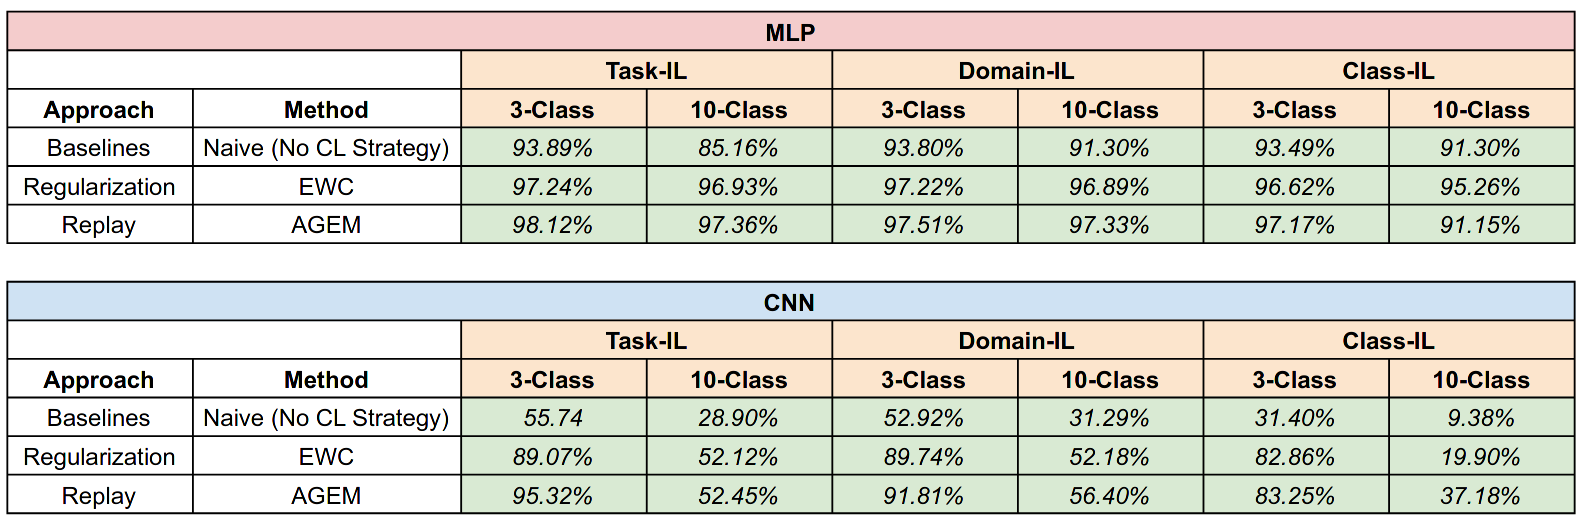
\includegraphics[width=1\linewidth]{results_table}
    \caption{Table of final results.}
	\label{fig:results_table}
\end{figure}

\begin{figure}[h]
	\centering
    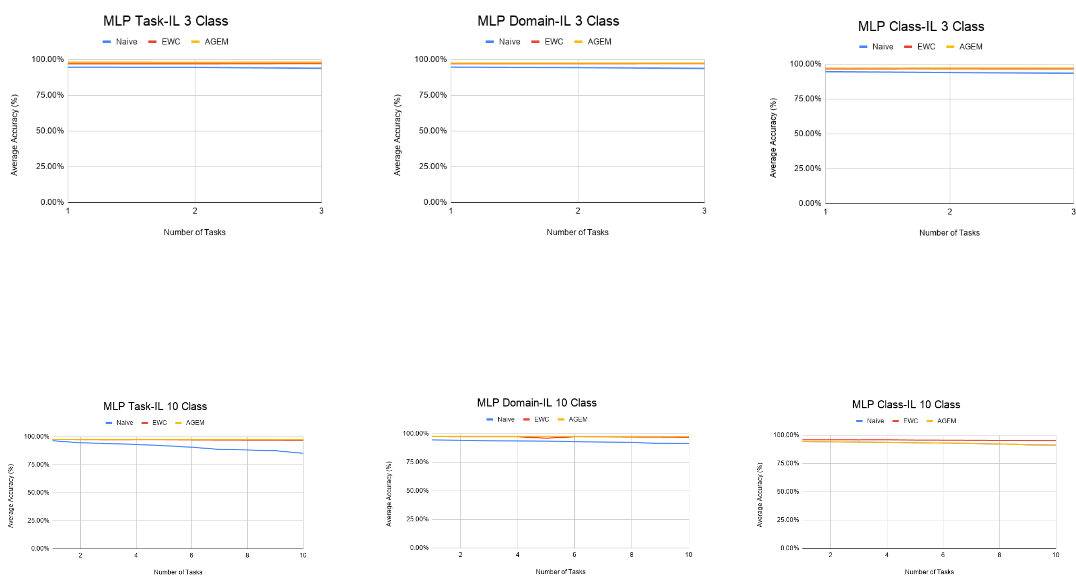
\includegraphics[width=1\linewidth]{res_1}
    \caption{MLP: Average accuracy computer after training on each task for all tasks.}
	\label{fig:res_1}
\end{figure}

\begin{figure}[h]
	\centering
    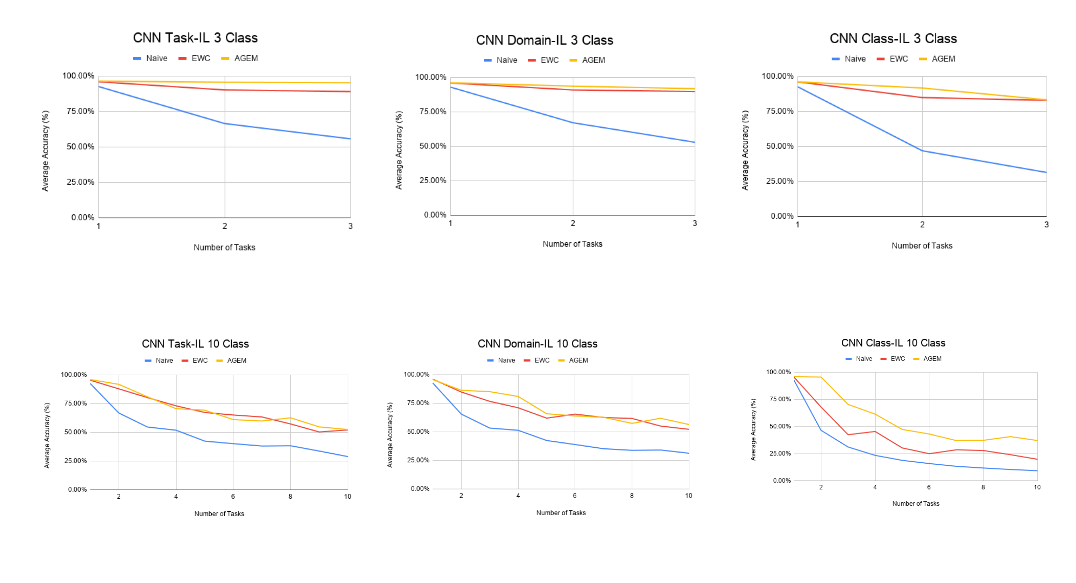
\includegraphics[width=1\linewidth]{res_2}
    \caption{CNN: Average accuracy computer after training on each task for all tasks.}
	\label{fig:res_2}
\end{figure}

%\section{Future Work}
%\section{Citations}
%\label{others}
%
%These instructions apply to everyone.
%
%\subsection{Citations within the text}
%
%The \verb+natbib+ package will be loaded for you by default.  Citations may be
%author/year or numeric, as long as you maintain internal consistency.  As to the
%format of the references themselves, any style is acceptable as long as it is
%used consistently.
%
%The documentation for \verb+natbib+ may be found at
%\begin{center}
%  \url{http://mirrors.ctan.org/macros/latex/contrib/natbib/natnotes.pdf}
%\end{center}
%Of note is the command \verb+\citet+, which produces citations appropriate for
%use in inline text.  For example,
%\begin{verbatim}
%   \citet{hasselmo} investigated\dots
%\end{verbatim}
%produces
%\begin{quote}
%  Hasselmo, et al.\ (1995) investigated\dots
%\end{quote}
%
%If you wish to load the \verb+natbib+ package with options, you may add the
%following before loading the \verb+neurips_2020+ package:
%\begin{verbatim}
%   \PassOptionsToPackage{options}{natbib}
%\end{verbatim}
%
%If \verb+natbib+ clashes with another package you load, you can add the optional
%argument \verb+nonatbib+ when loading the style file:
%\begin{verbatim}
%   \usepackage[nonatbib]{neurips_2020}
%\end{verbatim}
%
%As submission is double blind, refer to your own published work in the third
%person. That is, use ``In the previous work of Jones et al.\ [4],'' not ``In our
%previous work [4].'' If you cite your other papers that are not widely available
%(e.g., a journal paper under review), use anonymous author names in the
%citation, e.g., an author of the form ``A.\ Anonymous.''
%
%\subsection{Footnotes}
%
%Footnotes should be used sparingly.  If you do require a footnote, indicate
%footnotes with a number\footnote{Sample of the first footnote.} in the
%text. Place the footnotes at the bottom of the page on which they appear.
%Precede the footnote with a horizontal rule of 2~inches (12~picas).
%
%Note that footnotes are properly typeset \emph{after} punctuation
%marks.\footnote{As in this example.}
%
%\subsection{Figures}
%
%\begin{figure}
%  \centering
%  \fbox{\rule[-.5cm]{0cm}{4cm} \rule[-.5cm]{4cm}{0cm}}
%  \caption{Sample figure caption.}
%\end{figure}
%
%All artwork must be neat, clean, and legible. Lines should be dark enough for
%purposes of reproduction. The figure number and caption always appear after the
%figure. Place one line space before the figure caption and one line space after
%the figure. The figure caption should be lower case (except for first word and
%proper nouns); figures are numbered consecutively.
%
%You may use color figures.  However, it is best for the figure captions and the
%paper body to be legible if the paper is printed in either black/white or in
%color.
%
%\subsection{Tables}
%
%All tables must be centered, neat, clean and legible.  The table number and
%title always appear before the table.  See Table~\ref{sample-table}.
%
%Place one line space before the table title, one line space after the
%table title, and one line space after the table. The table title must
%be lower case (except for first word and proper nouns); tables are
%numbered consecutively.
%
%Note that publication-quality tables \emph{do not contain vertical rules.} We
%strongly suggest the use of the \verb+booktabs+ package, which allows for
%typesetting high-quality, professional tables:
%\begin{center}
%  \url{https://www.ctan.org/pkg/booktabs}
%\end{center}
%This package was used to typeset Table~\ref{sample-table}.
%
%\begin{table}
%  \caption{Sample table title}
%  \label{sample-table}
%  \centering
%  \begin{tabular}{lll}
%    \toprule
%    \multicolumn{2}{c}{Part}                   \\
%    \cmidrule(r){1-2}
%    Name     & Description     & Size ($\mu$m) \\
%    \midrule
%    Dendrite & Input terminal  & $\sim$100     \\
%    Axon     & Output terminal & $\sim$10      \\
%    Soma     & Cell body       & up to $10^6$  \\
%    \bottomrule
%  \end{tabular}
%\end{table}
%
%\section{Final instructions}
%
%Do not change any aspects of the formatting parameters in the style files.  In
%particular, do not modify the width or length of the rectangle the text should
%fit into, and do not change font sizes (except perhaps in the
%\textbf{References} section; see below). Please note that pages should be
%numbered.
%
%\section{Preparing PDF files}
%
%Please prepare submission files with paper size ``US Letter,'' and not, for
%example, ``A4.''
%
%Fonts were the main cause of problems in the past years. Your PDF file must only
%contain Type 1 or Embedded TrueType fonts. Here are a few instructions to
%achieve this.
%
%\begin{itemize}
%
%\item You should directly generate PDF files using \verb+pdflatex+.
%
%\item You can check which fonts a PDF files uses.  In Acrobat Reader, select the
%  menu Files$>$Document Properties$>$Fonts and select Show All Fonts. You can
%  also use the program \verb+pdffonts+ which comes with \verb+xpdf+ and is
%  available out-of-the-box on most Linux machines.
%
%\item The IEEE has recommendations for generating PDF files whose fonts are also
%  acceptable for NeurIPS. Please see
%  \url{http://www.emfield.org/icuwb2010/downloads/IEEE-PDF-SpecV32.pdf}
%
%\item \verb+xfig+ "patterned" shapes are implemented with bitmap fonts.  Use
%  "solid" shapes instead.
%
%\item The \verb+\bbold+ package almost always uses bitmap fonts.  You should use
%  the equivalent AMS Fonts:
%\begin{verbatim}
%   \usepackage{amsfonts}
%\end{verbatim}
%followed by, e.g., \verb+\mathbb{R}+, \verb+\mathbb{N}+, or \verb+\mathbb{C}+
%for $\mathbb{R}$, $\mathbb{N}$ or $\mathbb{C}$.  You can also use the following
%workaround for reals, natural and complex:
%\begin{verbatim}
%   \newcommand{\RR}{I\!\!R} %real numbers
%   \newcommand{\Nat}{I\!\!N} %natural numbers
%   \newcommand{\CC}{I\!\!\!\!C} %complex numbers
%\end{verbatim}
%Note that \verb+amsfonts+ is automatically loaded by the \verb+amssymb+ package.
%
%\end{itemize}
%
%If your file contains type 3 fonts or non embedded TrueType fonts, we will ask
%you to fix it.
%
%\subsection{Margins in \LaTeX{}}
%
%Most of the margin problems come from figures positioned by hand using
%\verb+\special+ or other commands. We suggest using the command
%\verb+\includegraphics+ from the \verb+graphicx+ package. Always specify the
%figure width as a multiple of the line width as in the example below:
%\begin{verbatim}
%   \usepackage[pdftex]{graphicx} ...
%   \includegraphics[width=0.8\linewidth]{myfile.pdf}
%\end{verbatim}
%See Section 4.4 in the graphics bundle documentation
%(\url{http://mirrors.ctan.org/macros/latex/required/graphics/grfguide.pdf})
%
%A number of width problems arise when \LaTeX{} cannot properly hyphenate a
%line. Please give LaTeX hyphenation hints using the \verb+\-+ command when
%necessary.
%
%
%\section*{Broader Impact}
%
%Authors are required to include a statement of the broader impact of their work, including its ethical aspects and future societal consequences. 
%Authors should discuss both positive and negative outcomes, if any. For instance, authors should discuss a) 
%who may benefit from this research, b) who may be put at disadvantage from this research, c) what are the consequences of failure of the system, and d) whether the task/method leverages
%biases in the data. If authors believe this is not applicable to them, authors can simply state this.
%
%Use unnumbered first level headings for this section, which should go at the end of the paper. {\bf Note that this section does not count towards the eight pages of content that are allowed.}
%
%\begin{ack}
%Use unnumbered first level headings for the acknowledgments. All acknowledgments
%go at the end of the paper before the list of references. Moreover, you are required to declare 
%funding (financial activities supporting the submitted work) and competing interests (related financial activities outside the submitted work). 
%More information about this disclosure can be found at: \url{https://neurips.cc/Conferences/2020/PaperInformation/FundingDisclosure}.
%
%
%Do {\bf not} include this section in the anonymized submission, only in the final paper. You can use the \texttt{ack} environment provided in the style file to autmoatically hide this section in the anonymized submission.
%\end{ack}

\medskip
\bibliography{references}

% \section*{References}
% 
% References follow the acknowledgments. Use unnumbered first-level heading for
% the references. Any choice of citation style is acceptable as long as you are
% consistent. It is permissible to reduce the font size to \verb+small+ (9 point)
% when listing the references.
% {\bf Note that the Reference section does not count towards the eight pages of content that are allowed.}
% \medskip
% 
% \small
% 
% [1] Alexander, J.A.\ \& Mozer, M.C.\ (1995) Template-based algorithms for
% connectionist rule extraction. In G.\ Tesauro, D.S.\ Touretzky and T.K.\ Leen
% (eds.), {\it Advances in Neural Information Processing Systems 7},
% pp.\ 609--616. Cambridge, MA: MIT Press.
% 
% [2] Bower, J.M.\ \& Beeman, D.\ (1995) {\it The Book of GENESIS: Exploring
%   Realistic Neural Models with the GEneral NEural SImulation System.}  New York:
% TELOS/Springer--Verlag.
% 
% %[3] Hasselmo, M.E., Schnell, E.\ \& Barkai, E.\ (1995) Dynamics of learning and
% %recall at excitatory recurrent synapses and cholinergic modulation in rat
% %hippocampal region CA3. {\it Journal of Neuroscience} {\bf 15}(7):5249-5262.
% 
% [4] Hassabis, Demis, et al. "Neuroscience-inspired artificial intelligence." Neuron 95.2 (2017): 245-258.

\end{document}
